\documentclass[12pt,fleqn]{article}
\setlength{\parindent}{0pt}
\usepackage{graphicx}
\usepackage{cancel}
\usepackage{listings}
\usepackage[latin5]{inputenc}
\setlength{\parskip}{8pt}
\setlength{\parsep}{0pt}
\setlength{\headsep}{0pt}
\setlength{\topskip}{0pt}
\setlength{\topmargin}{0pt}
\setlength{\topsep}{0pt}
\setlength{\partopsep}{0pt}
\setlength{\mathindent}{0cm}

\begin{document}
Piksel Takibi, Optik Akis, Lucas Kanade Algoritmasi

Hareket halindeki bir kameranin aldigi goruntulerdeki herhangi bir pikseli
nasil takip ederiz? 

Matematiksel olarak temsil etmek gerekirse, zamana gore degisen 2 boyutlu
goruntuyu bir fonksiyon olarak dusunelim, ki bu fonksiyonun degerleri
ayriksal olarak, imajin ta kendisi. Bir $I(x(t),y(t),t)$ fonksiyonu piksel
degerlerini veriyor. Bu fonksiyonda $x,y$ ekran kordinatlarina tekabul
ediyor, $t$ ise zaman, 1,2,.. gibi degerleri var, mesela $I(100,200,1)$,
bize 1. fotograftaki $x=100,y=200$ kordinatlarindaki piksel degerini
verecek. 

$x,y$ degiskenleri parametrize edildi, bir noktayi takip etmek istiyoruz
cunku, ve $t$'ye gore bu takip edilen noktanin $x,y$ kordinatlari belli bir
gidisat yonunde degisiyor.

O zaman su faraziyeyi yaparak problemimizi kolaylastirabiliriz. Diyelim ki
takip edilen bir nokta, goruldugu her karede ayni piksel rengindedir. Bu
cok siradisi bir faraziye degil, resim karelerinden bir araba geciyor, ve
bu arabanin uzerindeki piksellerin renkleri, en azindan iki kare arasinda
degismiyor. Isik seviyesi, golgede olma, vs. gibi durumlarda biraz
degisebilir, fakat basitlestirme amaciyla bu faraziye ise yarar.

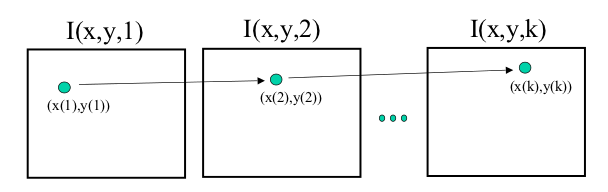
\includegraphics[height=3cm]{disp2.png}

Bir diger faraziye, kameralar hareket ettiklerinde alinan iki goruntu
arasindaki tum piksellerin yer degisimi genellikle ayni yonde olmasidir. Bu
degisim yonunu $<u,v>$ vektoru olarak gorebiliriz, ve bu degiskenler iki
goruntu arasindaki degisimde tum pikseller icin ayni olacaktir. Kamarayi
saga hareket ettiriyoruz, ve goruntudeki tum pikseller sola dogru
gidiyorlar. 

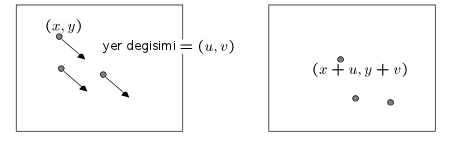
\includegraphics[height=3cm]{disp.png}

Tum bunlari modelimizde nasil kullaniriz? 

Takip edilen nokta her karede ayni renkte ise, su ifade dogru demektir 

\[ I(x(t),y(t),t) = \textrm{ sabit } \]

Eger bu fonksiyonun zamana gore turevini alirsak

\[ \frac{d \ I(x(t),y(t),t)}{dt} = 0\]

sonucu gelir. Esitligin sagi sifir, cunku bir sabitin turevini aldik. Sol
tarafa Zincirleme Kanununu uygularsak, 

\[ \frac{\partial I}{\partial x}\frac{dx}{dt} +
\frac{\partial I}{\partial y}\frac{dy}{dt} +
\frac{\partial I}{\partial t} = 0
\]

Bu formulde $dx/dt$ ve $dy/dt$, hareket halindeki (zaman gecerken) noktanin
sonsuz kucuklukteki ne kadar yer degimi. Ayriksal baglamda arka arkaya iki
kare icindeki yer degisimi. O zaman,

\[ \frac{dx}{dt}, \frac{dy}{dt} = u, v \]

Alttakiler ise mesafesel (spatial) gradyanlardir, bunlarin nasil
hesaplanacagini cok iyi biliyoruz! 

\[ 
\frac{\partial I}{\partial x}, \frac{\partial I}{\partial y}
 \]

Alttaki ise resim karelerinin zamana gore turevi

\[ 
\frac{\partial I}{\partial t}
 \]

Daha derli toplu olarak gostermek gerekirse ana formul nihai olarak soyle

\[ I_x u + I_y v + I_t = 0 \]

ya da

\[ 
\nabla I \cdot <u, v> = -I_t
 \]

Peki bizim sectigimiz (takip edecegimiz) bir piksel icin $u,v$'yi nasil
hesaplayacagiz? Ustteki formulu hem takip ettigimiz, hem de onun
etrafindaki pikseller icin yazarsak, ve bu sistemi cozersek, sonuca
varabiliriz. Boylece iki tane bilinmeyenimiz olacak, ama pek cok formul
gececek. Veriler gurultulu oldugu icin, aslinda bilinmeyenden ``daha
fazla'' formul elde etmek iyi, boylece elimizdeki denklem sistemi cok
esitlige sahip (overdetermined) bir hale gelecek, ve bu tur sistemleri En
Az Kareler (Least Squares) yontemi ile cozmeyi biliyoruz. Tum bu
denklemleri biraraya koyunca soyle bir sistem ortaya cikar

\[ 
\left[\begin{array}{cc}
I_x(p_1) & I_y(p_1) \\
I_x(p_2) & I_y(p_1) \\
\vdots & \vdots \\
I_x(p_k) & I_y(p_k) 
\end{array}\right]
\left[\begin{array}{r}
u \\
v
\end{array}\right] = 
-
\left[\begin{array}{c}
I_t(p_1) \\
I_t(p_2) \\
\vdots \\
I_t(p_k) 
\end{array}\right]
 \]

Bu sistemi

\[ A \ d = b \]

olarak gosterebiliriz. Sol tarafi $A^T$ ile carpalim

\[ A^TA \ d = A^Tb \]

Eger $A^TA$'nin matris tersini iki tarafla carparsak, $d$ yanliz kalir, ve
sonuc elde edilir. Bu denklemi Python Numpy icinde \verb!pinv! kullanarak
cozeriz. 

Test icin uc tane resim kullandik, bu resimlerden \verb!flow1-bw-0.png!
baslangic resmi, bu resmin ortasindaki objeleri GIMP kullanarak elle
kopyaladik, bir ust sag capraza dogru, bir alt sol capraza dogru, ve iki
yeni resim elde ettik (\verb!upright.png!, \verb!dleft.png!). Takip edilen
nokta gri dortgenin alt sol kosesinde. Lucas Kanade algoritmasi bu noktayi
takip ederek, yesil ile isaretledi.

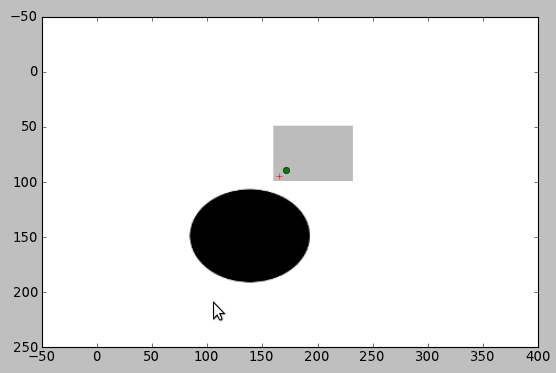
\includegraphics[height=4cm]{res1.png}

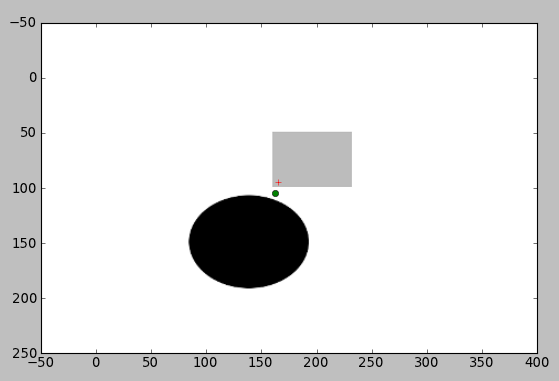
\includegraphics[height=4cm]{res2.png}

\lstinputlisting[language=Python]{deriv.py}

\lstinputlisting[language=Python]{lk.py}

Kaynaklar

R. Collins Ders Notlari, www.cse.psu.edu/~rcollins/CSE486


\end{document}
